\documentclass[11pt,fleqn]{exam}
\usepackage[utf8]{inputenc}

\usepackage[margin=1in]{geometry}
\usepackage{amsmath,amssymb}
\usepackage{gensymb}
\usepackage{multicol}
\usepackage{float}
\usepackage{graphicx}
\usepackage{units,icomma}
\usepackage[colorlinks,linkcolor=blue,urlcolor=blue]{hyperref}
\usepackage[margin=1.5cm]{caption}

\usepackage[shortlabels]{enumitem}

\hyphenation{
  chro-no-ampe-ro-met-ric
  ber-dia-me-ter
  de-ngan
  me-nem-pati
  mic-ro-graphs}

\renewcommand{\figurename}{Gambar.}
\def\equationautorefname{Persamaan}
\newcommand{\class}{OLIMPIADE ASTRONOMI}
\newcommand{\term}{Tingkat Propinsi - 2017}
\newcommand{\examnum}{OSP Astronomi 2017}
%\newcommand{\examdate}{11/02/2014}
%\newcommand{\timelimit}{120 Minutes}

\pagestyle{head}
\firstpageheader{}{}{}
\runningheader{\examnum}{}{Halaman \thepage\ dari \numpages}
\runningheadrule


\begin{document}

\noindent
\begin{tabular*}{\textwidth}{l @{\extracolsep{\fill}} r @{\extracolsep{6pt}} l}
\textbf{\class} \\% & \textbf{Name:} & \makebox[2in]{\hrulefill}\\
\textbf{\term}  %&&\\
%\textbf{\examnum} &&\\
%\textbf{\examdate} &&\\
%\textbf{Time Limit: \timelimit} & Teaching Assistant & \makebox[2in]{\hrulefill}
\end{tabular*}\\
\rule[2ex]{\textwidth}{2pt}

\noindent
\begin{tabular}{ll}
Copyright (c) 2017 & Ridlo W. Wibowo (ridlo.w.wibowo@gmail.com)\\
                   & Sulistiyowati (sulis.astro08@gmail.com)
\end{tabular}

\vspace{0.3cm}
\noindent
Solusi ini dibuat tanpa jaminan kesesuaian dengan solusi resmi dari juri olimpiade sains bidang Astronomi. Pengguna boleh menyebarluaskan dan/atau memodifikasi solusi ini dengan mencantumkan sumber asli. Hak cipta soal ada pada Kemendiknas dan dilindungi undang-undang.

\vspace{0.4cm}
\noindent
\rule[2ex]{\textwidth}{1.5pt}

\textbf{SOAL PILIHAN GANDA}

\begin{questions}
\question Angin Matahari di dekat orbit Bumi memiliki kecepatan 400 km/detik dan mengandung 10 proton per cm\textsuperscript{3}. Jika dua besaran tersebut dianggap selalu tetap hingga umur Matahari saat ini,  yaitu 4,5 milyar tahun, maka massa Matahari yang telah hilang karena angin Matahari adalah sebesar
\begin{choices}
\choice $0,285 M_{\odot}$
\choice $0,675 M_{\odot}$
\choice $1,34\times 10^{-4} M_{\odot}$
\choice $5,944\times 10^{-11} M_{\odot}$
\choice $5,025\times 10^{-24} M_{\odot}$
\end{choices}

\textit{Jawaban: C}\\
$v_p=400$ km/detik $=4\times10^5$ meter/detik\\
$n_p=10$ proton per cm\textsuperscript{3}$= 10^{7}$ proton per per m\textsuperscript{3}\\
$m_p=1,6726\times 10^{-27}$ kg\\
$\rho_p=m_p n_p=1,6726\times 10^{-20}$ kg/m\textsuperscript{3}\\
$\Delta t=4,5\times 10^9$ tahun $=1,42\times 10^{17}$ detik\\
$d_{\odot\oplus}=1,49597870\times10^{11}$ meter\\
$M_{\odot \text{loss}}=$ \ldots ?\\

Massa total yang telah hilang:
$$M_{\odot loss}=\dot{m}_{\odot \text{loss}}\Delta t$$ 
$\dot{m}_{\odot \text{loss}}$ menyatakan massa yang hilang per satuan waktu; analogi debit dalam kasus fluida:
$$\dot{m}_{\odot \text{loss}}=\rho_p v_p A \quad \text{kg/s}$$
$\rho$ menyatakan kerapatan proton di dekat Bumi, sedangkan $A$ menyatakan luas penampang yang ditembus proton di dekat Bumi, $A=4\pi d_{\odot\oplus}^2$
maka,
\begin{eqnarray*}
M_{\odot \text{loss}} = \rho_p v_p 4\pi d_{\odot\oplus}^2 \Delta t = 6,68\times 10^{25} \text{  kg} = 1,34\times 10^{-4}M_{\odot}
\end{eqnarray*}


\vspace{0.3cm}
\question Berapa periode rotasi ekuator sebuah bintang katai putih yang berukuran sama dengan Planet Bumi dan memiliki massa sama dengan massa Matahari? (Anggaplah momentum sudut sebesar momentum sudut Matahari)
\begin{choices}
\choice 33 hari
\choice 3,3 hari
\choice 3,3 jam
\choice 3,3 menit
\choice 3,3 detik
\end{choices}

\textit{Jawaban: D} \\
$R_*=R_{\oplus}=6378$ km\\
$M_*=M_{\odot}$\\
$L_*=L_{\odot}$\\
Periode rotasi bintang katai putih ($P_*$) dengan menganggap bintang katai putih dan Matahari sebagai benda pejal:
\begin{eqnarray*}
L_*&=&L_{\odot}\\
I_*\omega_* &=& I_{\odot}\omega_{\odot}\\
\frac{2}{5}M_*R_*^2 \frac{2\pi}{P_*}&=&\frac{2}{5}M_{\odot}R_{\odot}^2\frac{2\pi}{P_{\odot}}\\
P_*&=& \frac{M_*}{M_{\odot}}\left(\frac{R_*}{R_{\odot}}\right)^2P_{\odot}\\
P_*&=&\left(\frac{R_*}{R_{\odot}}\right)^2P_{\odot}\\
P_*&=& 2,27\times 10^{-3}\quad \text{hari}\quad=\quad3,3 \quad \text{menit}
\end{eqnarray*}

\vspace{0.3cm}
\question Tidak teramatinya aurora di Planet Venus disebabkan oleh
\begin{choices}
\choice tidak ada oksigen di atmosfer Venus
\choice atmosfer Venus terlalu tebal
\choice medan magnet di Venus sangat lemah
\choice temperatur permukaan Venus yang tinggi
\choice jarak Venus terlalu dekat dengan Matahari
\end{choices}

\textit{Jawaban: C} \\
Aurora terjadi karena interaksi antara partikel bermuatan dari angin Matahari dengan medan magnet planet. Akibat interaksi, partikel dengan arah datang tertentu akan terseret mengikuti medan magnet planet mendekati permukaan planet. Ketika berada di dekat permukaan planet, partikel bermuatan akan bertumbukan dengan molekul di atmosfer planet kemudian mengalami transfer energi yang tampak sebagai cahaya aurora. Venus memiliki atmosfer tebal, tetapi medan magnetnya lemah sekali.

Sehingga pilihan yang paling tepat C.\\


\vspace{0.3cm}
\question Kita tidak mengharapkan akan dapat mempelajari evolusi kehidupan di planet yang mengelilingi bintang bermassa besar, karena
\begin{choices}
\choice bintang bermassa besar luminositasnya amat tinggi
\choice kala hidup bintang bermassa besar terlalu pendek
\choice planet pada bintang bermassa besar terlalu panas untuk makhluk hidup
\choice orbit planet pada bintang bermassa besar tidak akan stabil
\choice semua alasan di atas benar
\end{choices}

\textit{Jawaban: B} \\
Meskipun luminositas besar dan temperatur efektif tinggi, akan selalu ada \textit{habitable zone} yang bisa ditemukan di sekitar bintang. Sehingga pilihan yang kaitannya dengan luminositas dan temperatur menjadi tidak relevan.

Kestabilan orbit suatu benda lebih dipengaruhi oleh jumlah benda bermassa signifikan yang terlibat dalam interaksi. Pernyataan tentang orbit planet pada bintang bermassa besar belum tentu valid.

Dengan kala hidup bintang pendek, kita tidak bisa berharap kehidupan memiliki kesempatan untuk berkembang.

Sehingga pilihan yang paling tepat B.\\

\vspace{0.3cm}
\question Objek di bawah ini yang dapat digunakan untuk menentukan pusat Galaksi kita adalah
\begin{choices}
\choice bintang muda
\choice awan antar bintang
\choice gugus bola
\choice gas Hidrogen dingin
\choice bintang bermassa 20 $M_{\odot}$
\end{choices}

\textit{Jawaban: C} \\
Bintang muda tersebar di sepanjang piringan Galaksi. Di piringan Galaksi tersebar pula banyak materi/awan antar bintang sehingga pengamatan sulit dilakukan di sepanjang piringan Galaksi karena kuatnya serapan oleh materi antar bintang tersebut. Gugus bola adalah objek terang yang distribusinya isotropik dari pusat Galaksi, dengan mengamati sebaran posisi gugus bola yang ada di semua arah relatif terhadap pusat Galaksi, posisi pusat Galaksi dapat ditentukan. Gas Hidrogen dingin lebih cocok digunakan untuk menentukan kecepatan rotasi Galaksi. Bintang bermassa 20 $M_{\odot}$ (besar) biasanya kala hidupnya pendek sehingga akan lebih jarang diamati.

Sehingga jawaban yang paling tepat C.\\

\vspace{0.3cm}
\question Kurva kecepatan radial dari sebuah sistem bintang ganda diberikan pada gambar di bawah ini (kecepatan radial dari masing-masing bintang dinyatakan terhadap fase orbitnya). Pernyataan manakah di bawah ini yang benar terkait dengan karakteristik dari kecepatan radial ($V_A$, $V_B$), periode orbital ($T_A$, $T_B$), dan massa ($M_A$, $M_B$) dari sistem bintang ganda tersebut?
\begin{figure}[h!]
\centering
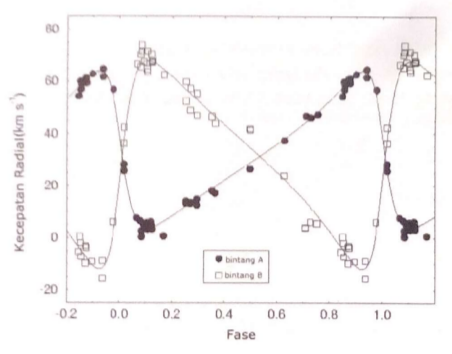
\includegraphics[width=0.5\textwidth]{no6.png}
\end{figure}

\begin{choices}
\choice $V_A > V_B, T_A > T_B, M_A > M_B$
\choice $V_A < V_B, T_A = T_B, M_A > M_B$
\choice $V_A < V_B, T_A < T_B, M_A < M_B$
\choice $V_A > V_B, T_A = T_B, M_A < M_B$
\choice $V_A > V_B, T_A = T_B, M_A > M_B$
\end{choices}

\textit{Jawaban: B} \\
Komponen sistem bintang ganda sudah seyogyanya memiliki periode sama, gambar pada soal pun menunjukkan demikian. Amplitudo bintang A lebih kecil daripada bintang B, artinya kecepatan bintang A lebih kecil dibanding bintang B. Bintang A mengorbit pusat massa pada jarak lebih dekat dibanding bintang B. Artinya, massa bintang A lebih besar daripada bintang B.

Sehingga jawaban yang tepat B.\\


\vspace{0.3cm}
\question Adanya zaman es (\textit{pleistocene}) di Bumi diyakini para ilmuwan disebabkan secara dominan oleh
\begin{choices}
\choice adanya perubahan dalam luaran energi dari Matahari
\choice tingkat aktivitas gunung berapi yang tinggi menyebabkan \textit{outgassing} dari CO\textsubscript{2} di atmosfer
\choice pergerakan lempeng benua
\choice presesi sumbu rotasi Bumi dan perubahan kelonjongan orbit Bumi
\choice Bumi ditabrak oleh asteroid raksasa
\end{choices}

\textit{Jawaban: D} \\
Perubahan insolasi Matahari yang datang ke Bumi diduga kuat merupakan penyebab terjadinya zaman es terakhir (\textit{pleistocene}). Zaman es terjadi beberapa kali sepanjang sejarah Bumi. \textit{Pleistocene} hanya merupakan salah satunya saja. Penjelasan lebih lanjut dapat dibaca di \url{http://culter.colorado.edu/~saelias/glacier.html} dan \url{https://geology.utah.gov/map-pub/survey-notes/glad-you-asked/ice-ages-what-are-they-and-what-causes-them/}.

Sehingga jawaban paling tepat D.


\vspace{0.3cm}
\question Diketahui percepatan relatif sebuah wahana antariksa terhadap percepatan gravitasi Bumi adalah sebesar 2 m/detik\textsuperscript{2}. Massa wahana itu adalah sebesar 13150 kg. Hitung berapa lama wahana tersebut bisa mencapai kecepatan lepas Bumi jika awalnya wahana berada dalam keadaan diam kemudian bergerak tegak lurus terhadap permukaan Bumi
\begin{choices}
\choice 2 detik
\choice 250 detik
\choice 90 menit
\choice 120 menit
\choice 120 jam
\end{choices}

\textit{Jawaban: } Tidak ada

\begin{enumerate}[a)]
\item Cara pertama yang salah: percepatan gerak roket dianggap tetap sebesar 2 m/s$^2$ ke atas; perubahan ketinggian terhadap kecepatan lepas diabaikan.
\begin{eqnarray*}
v = v_0 + at &=& \sqrt{\frac{2GM}{R^2}}\\
2t &=& 11200\\
t &=& 5600\text{   s} = 93,33 \text{  menit}
\end{eqnarray*}
Ketinggian yang sudah dicapai selama 93,33 menit adalah 31360 km, tentu hal ini tidak dapat diabaikan!

\item Cara kedua yang masih salah: percepatan gerak roket dianggap tetap sebesar 2 m/s$^2$ ke atas; memasukkan faktor perubahan ketinggian terhadap nilai kecepatan lepas yang diperlukan ke dalam persamaan.
\begin{eqnarray*}
v = v_0 + at &=& \sqrt{\frac{2GM}{R+(h_0 + v_0 t + \frac{1}{2} a t^2)}}\\
a^2 t^2 &=& \frac{2GM}{R + \frac{1}{2} a t^2}\\
\frac{1}{2} a^3 t^4 + R a^2 t^2 - 2GM &=& 0, \qquad \text{gunakan  } x = t^2\\
\frac{1}{2} a^3 x^2 + R a^2 x - 2GM &=& 0, \qquad \text{dapat dicari solusinya menggunakan rumus } abc\\
t &=& \sqrt{x} = 56,055 \quad \text{menit}
\end{eqnarray*}

\item Kedua cara di atas mengasumsikan percepatan gerak yang konstan, padahal dengan asumsi roket pendorongnya yang ajeg, maka seharusnya besarnya gaya yang bernilai konstan (bukan percepatan). Ketika wahana bergerak naik dengan nilai gaya yang tetap, \textit{padahal nilai $g$ berubah seiring dengan bertambah tingginya wahana}, maka percepatan geraknya juga seharusnya berubah. Apalagi ditambah ketika bergerak ada sejumlah massa yang dibuang, beratnya pun ikut berubah.
\begin{eqnarray*}
F = m(t) (g(t) + a(t)) \quad \text{(asumsi gaya F bernilai konstan selama wahana bergerak)}
\end{eqnarray*}

\end{enumerate}



\vspace{0.3cm}
\question Foton dengan panjang gelombang datang sebesar 0,2\AA~mengalami kehilangan energi. Panjang gelombang foton setelah kehilangan 73\% energi adalah
\begin{choices}
\choice $9,9\times 10^{-11}$ m
\choice $7,4\times 10^{-11}$ m
\choice $6,5\times 10^{-11}$ m
\choice $3,4\times 10^{-11}$ m
\choice $2,0\times 10^{-11}$ m
\end{choices}

\textit{Jawaban: B} \\
$\lambda_0=0,2$ \AA, $E_0=\frac{hc}{\lambda_0}$. 

Setelah kehilangan energi 73\%: 
\begin{eqnarray*}
E &=& (100\%-73\%)E_0\\
\frac{hc}{\lambda} &=& 27\% \frac{hc}{\lambda_0}\\
\lambda &=& \frac{\lambda_0}{27\%} = 0,74 \text{ \AA} = 7,4\times 10^{-11} \quad \text{m}
\end{eqnarray*}


\vspace{0.3cm}
\question Tabel berikut adalah data untuk Bintang GI 581 yang memiliki sistem keplanetan

\begin{table}[h!]
\centering
\caption*{Data GI 581}
\begin{tabular}{|c|c|c|c|}
\hline
Kelas spektrum & Magnitudo visual & Magnitudo mutlak bolometrik & Jarak ke Bumi \\
\hline
M3 & 10,55 & 9,58 & 6,21 pc \\
\hline
\end{tabular}
\end{table}

Beberapa planet di antaranya ditemukan berada pada zona yang dapat dihuni (\textit{habitable zone}, \textit{HZ}) dari bintang. \textit{Habitable zone} adalah zona seputar bintang dengan tekanan atmosfer sedemikian rupa sehingga dapat ditemukan air berwujud cair di permukaan planet. Rumus empirik untuk batas dalam dan batas luar masing-masing adalah

\begin{eqnarray*}
HZ_{in} &=& 0,95\sqrt{\frac{L_*}{L_{\odot}}} \quad \text{au} \\
HZ_{out} &=& 1,37\sqrt{\frac{L_*}{L_{\odot}}} \quad \text{au}
\end{eqnarray*}

dengan $L_*$ dan $L_{\odot}$ adalah luminositas bintang dan Matahari. Nilai batas dalam dan batas luar untuk GI 581 dalam satuan au masing-masing adalah
\begin{choices}
\choice 0,1 dan 0,14
\choice 0,044 dan 0,095
\choice 0,054 dan 0,078
\choice 0,09 dan 0,20
\choice 0,95 dan 1,15
\end{choices}

\textit{Jawaban: A}\\
Tentukan terlebih dahulu luminositas bintang $L_*$ dengan memanfaatkan magnitudo mutlak bolometrik bintang $M_{bol}$ dan magnitudo mutlak bolometrik Matahari $M_{bol \odot}$.
\begin{eqnarray*}
M_{bol}-M_{bol \odot} &=& -2,5\log\frac{L_*}{L_{\odot}}\\
9,58-4,72 &=& -2,5\log\frac{L_*}{L_{\odot}}\\
L_* &=& 0,01L_{\odot}
\end{eqnarray*}
\begin{eqnarray*}
HZ_{in} &=& 0,95\sqrt{\frac{0,01L_{\odot}}{L_{\odot}}} = 0,101\\
HZ_{out} &=& 1,37\sqrt{\frac{0,01L_{\odot}}{L_{\odot}}}=0,146
\end{eqnarray*}

\vspace{0.3cm}
\question Daya pisah (\textit{resolution}) suatu teleskop dengan bukaan $D$ dan panjang fokus $f$ dapat ditingkatkan dengan cara
\begin{choices}
\choice mengecilkan diameter teleskop
\choice mengamati objek pada panjang gelombang yang lebih pendek
\choice mengamati objek pada panjang gelombang yang lebih panjang
\choice menambah panjang fokus
\choice memperpendek panjang fokus
\end{choices}

\textit{Jawaban: B}\\
Daya pisah $\theta$ suatu teleskop berdiameter $D$ dapat dirumuskan secara matematis:
$$\theta\propto\frac{\lambda}{D},$$ 
dengan $\lambda$ menyatakan panjang gelombang yang digunakan untuk mengamati objek. Meningkatnya daya pisah diindikasikan dengan mengecilnya nilai $\theta$. Teleskop yang baik memiliki $\theta$ kecil, artinya dapat mengidentifikasi dua objek yang terpisah sejauh $\theta$ di langit sebagai dua sumber cahaya terpisah.

\vspace{0.5cm}
\textbf{Untuk satu soal berikut ini (No 12), jawablah}
\begin{choices}
\choice \textbf{jika 1, 2, dan 3 benar}
\choice \textbf{jika 1 dan 3 benar}
\choice \textbf{jika 2 dan 4 benar}
\choice \textbf{jika 4 saja benar}
\choice \textbf{jika semua benar}
\end{choices}

\vspace{0.3cm}
\question Pada bulan Februari tahun 2017, tim astronomi internasional menemukan tujuh eksoplanet yang mengelilingi sebuah bintang bernama TRAPPIST-1. Bintang bermassa $0,080 M_{\odot}$ ini memiliki jarak 39 tahun cahaya dari sistem Tata Surya. Tiga dari tujuh planetnya berada pada HZ (lihat soal 10) dan memiliki periode orbit berturut-turut 1,5, 2,5, dan 4 hari. Asumsikan orbit planet-planet tersebut berbentuk lingkaran dengan Bintang TRAPPIST-1 berada di pusatnya. Manakah pernyataan yang benar?
\begin{enumerate}
\item Jarak planet terdekat pertama ke Bintang TRAPPIST-1 adalah 0,026 au.
\item Jarak planet terdekat kedua ke Bintang TRAPPIST-1 adalah 0,084 au.
\item Sudut paralaks Bintang TRAPPIST-1 dari planetnya adalah 0,08 detik busur.
\item Periode sinodis antara planet pertama dan ketiga adalah 2,4 hari.
\end{enumerate}

\textit{Jawaban: D} \\
Penjelasan awal yang diberikan sebetulnya tidak mengindikasikan bahwa tiga planet tersebut adalah tiga planet terdekat. Dengan mengasumsikan ketiga planet di atas adalah tiga planet terdekat,
\begin{itemize}
\item Pernyataan pertama salah, seharusnya 0,011 au.
\begin{equation*}
a = \sqrt[3]{MT^2} = \sqrt[3]{0,08 \cdot \left(\frac{1,5}{365,25}\right)^2} = 0,011 \quad \text{au}
\end{equation*}
\item Pernyataan kedua salah, seharusnya 0,0155 au.
\begin{equation*}
a = \sqrt[3]{MT^2} = \sqrt[3]{0,08 \cdot \left(\frac{2,5}{365,25}\right)^2} = 0,0155 \quad \text{au}
\end{equation*}
\item Pernyataan ketiga kurang jelas maksudnya, apakah maksudnya paralaks horizon?
\item Pernyataan keempat benar,  2,4 hari.
\begin{eqnarray*}
T_{\sin} = \frac{T_1 T_2}{T_2 - T_1} = \frac{1,5 \cdot 4}{4 - 1,5} = 2,4 \quad \text{hari}
\end{eqnarray*}
\end{itemize}



\vspace{0.5cm}
\textbf{Gunakan petunjuk ini untuk menjawab tiga soal berikut (No. 13-15):}
\begin{choices}
\choice \textbf{Pernyataan pertama dan kedua benar serta memiliki hubungan sebab-akibat.}
\choice \textbf{Pernyataan pertama dan kedua benar, tetapi tidak memiliki hubungan sebab-akibat.}
\choice \textbf{Pernyataan pertama benar, sedangkan pernyataan kedua salah.}
\choice \textbf{Pernyataan pertama salah, sedangkan pernyataan kedua benar.}
\choice \textbf{Kedua pernyataan salah.}
\end{choices}

\vspace{0.3cm}
\question Posisi Matahari terbenam tampak lebih rendah daripada posisi sebenarnya.
\begin{center}
SEBAB
\end{center}
Cahaya Matahari mengalami refraksi ketika melewati atmosfer Bumi.\\

\textit{Jawaban: D} \\
Posisi Matahari terbenam tampak lebih tinggi daripada posisi sebenarnya karena cahayanya mengalami refraksi ketika melewati atmosfer Bumi.

Pernyataan pertama salah, pernyataan kedua benar.

\vspace{0.3cm}
\question Light exhibit polarization.
\begin{center}
BECAUSE
\end{center}
Light waves oscillate in the direction of their wave propagation.\\

\textit{Jawaban: C}\\
Electromagnetic radiation/light exhibit polarization. Electromagnetic radiation/light belongs to transversal waves, which oscillate in the direction perpendicular to the direction of their propagation.

First statement is true, second statement is wrong.

\vspace{0.3cm}
\question Warna galaksi spiral lebih biru daripada warna galaksi elips.
\begin{center}
SEBAB
\end{center}
Adanya garis-garis emisi dalam spektrum galaksi spiral menandakan terjadinya pembentukan bintang-bintang.\\

\textit{Jawaban: B} \\
Warna galaksi spiral lebih biru daripada warna galaksi elips karena galaksi spiral banyak memiliki populasi bintang muda. Garis-garis emisi dalam spektrum galaksi spiral menandakan terdapat banyak gas panas/terionisasi di galaksi tersebut yang mengindikasikan terjadinya pembentukan bintang-bintang.

Pernyataan pertama benar, pernyataan kedua benar, tidak saling berhubungan sebab akibat.

\vspace{0.5cm}
\textbf{Soal Isian Singkat}

\question Materi sebuah bintang bermassa $M=1,989\times 10^{30}$ kg dan beradius $R=6,96\times 10^8$ m dianggap memenuhi kondisi gas ideal dan sepenuhnya hanya mengandung hidrogen. Jumlah atom hidrogen di bintang tersebut adalah \ldots\ldots\ldots \\

\textit{Jawaban: }

Memenuhi kondisi gas ideal berarti tidak ada efek-efek `aneh' yang perlu kita tinjau :)

Jika bintang ini bermassa $1,989 \times 10^{30}$ kg, padahal ia tersusun atas Hidrogen dengan massa per atomnya adalah $1,6735 \times 10^{-27}$ kg, maka jumlah atom Hidrogennya adalah 
$$\frac{1,989 \times 10^{30}}{1,6735 \times 10^{-27}} = 1,1885 \times 10^{57}$$


\vspace{0.3cm}
\question Fluks sebuah bintang bermagnitudo $m=0$ adalah \ldots\ldots\ldots W/m\textsuperscript{2}.\\

\textit{Jawaban: } $2,692 \times 10^{-8}$

Luminositas Matahari, jarak, dan magnitudo semunya dapat ditemukan di daftar konstanta yang diberikan. Fluks Matahari diukur dari Bumi adalah
\begin{eqnarray*}
F &=& \frac{L}{4 \pi d^2} \\
  &=& \frac{3,9 \times 10^{26}}{4 \pi (1,49597870 \times 10^{11})^2} = 1386,77 \quad \text{W/m}^{2}
\end{eqnarray*}

Jika suatu bintang memiliki magnitudo semu $m = 0$, maka fluksnya sebesar
\begin{eqnarray*}
m - m_{\odot} &=& -2,5 \log\left(\frac{F}{F_{\odot}}\right)\\
0 + 26,78 &=& -2,5 \log\left(\frac{F}{1386,77}\right)\\
F &=&   2,692 \times 10^{-8} \quad \text{W/m}^{2}
\end{eqnarray*}


\vspace{0.3cm}
\question Dua lokasi di muka Bumi masing-masing berada pada $30\degree$ Lintang Selatan (LS) dan $45\degree$ Lintang Utara (LU). Kedua lokasi terpisah jarak sejauh 2126$\pi$ km. Beda bujur ($\Delta B_j$) kedua lokasi tersebut dalam satuan radian adalah \ldots\ldots\ldots\\

\textit{Jawaban: } Tidak mungkin, data yang diberikan salah.

Jarak dua lokasi dinyatakan dalam besarnya sudut di pusat Bumi,
\begin{equation*}
\theta = \frac{2126 \pi }{6378} = \frac{\pi}{3} \quad \text{rad} = 60\degree
\end{equation*}

Jarak ini terlalu kecil dan tidak sesuai dengan data lintang yang diberikan. Dari data lintang yang diberikan, jarak sudut minimum kedua lokasi adalah $75\degree$, yaitu ketika keduanya berada di bujur yang sama.\\

%Beda bujur kedua lokasi $\Delta B_j$ dapat ditentukan dengan persamaan segitiga bola,
%\begin{eqnarray*}
%\cos{(60\degree)} &=& \cos(90\degree + 30\degree) \cos(90\degree - 45\degree)  + \sin(90\degree + 30\degree) \sin(90\degree - 45\degree) \cos(\Delta B_j)\\
%\cos(\Delta B_j) &=& \frac{\cos{(60\degree}) - \cos(120\degree) \cos(45\degree)}{\sin(120\degree) \sin(45\degree)}\\
%\cos(\Delta B_j) &=& \frac{\frac{1}{2} - (-\frac{1}{2})(\frac{1}{2}\sqrt{2})}{(\frac{1}{2}\sqrt{3})(\frac{1}{2}\sqrt{2})} > 1 \qquad \text{Error!}
%\end{eqnarray*}

$^\star$Kecuali mereka berada di dalam tanah (radiusnya kurang dari radius Bumi) :P\\

\vspace{0.3cm}
\question Saat di perigee (jarak 356800 km), piringan Bulan purnama diamati sebesar 34,2 menit busur. Pada fase Bulan mati/baru di apogee, piringan Bulan diukur sebesar 30,0 menit busur. Sinar Matahari dianggap mengenai Bumi dan Bulan secara sejajar. Jarak Bulan pada fase $\frac{1}{2}$ adalah \ldots\ldots\ldots km.\\


\textit{Jawaban: } 382417,45

Diketahui:

Jarak terdekat bulan ($r_{\text{min}}$) = 356800 km

Jarak rata-rata Bumi-Bulan ($a$) = 384399 km

eksenstrisitas orbit Bulan dapat dicari,
\begin{eqnarray*}
r_{\text{min}} &=& a (1 - e)\\
e &=& 1 - \frac{r_{\text{min}}}{a} = 0,0718
\end{eqnarray*}

Karena Bulan purnama tepat saat perigee dan Bulan baru tepat pada saat apogee, maka dapat digambarkan posisiny sebagai berikut.

\begin{figure}[ht!]
\centering
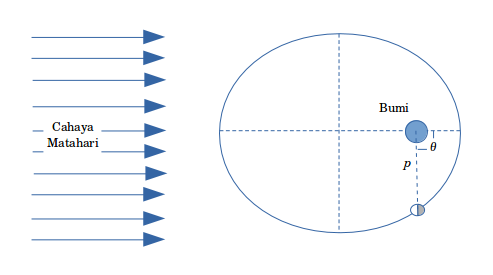
\includegraphics[width=0.7\textwidth]{19.png}
\end{figure}

Karena sinar Matahari dianggap mengenai Bumi dan Bulan secara sejajar (jarak Matahari cukup jauh dibanding jarak Bulan), maka posisi Bulan saat fase setengah pasti berada di semilatus rectum. Jaraknya dapat dicari dari persamaan elips,
\begin{eqnarray*}
r = \frac{a (1 - e^2)}{1 + e \cos{\theta}}
\end{eqnarray*}
Saat berada di posisi semilatus rectum ($\theta = 90\degree$), jarak Bulan menjadi,
\begin{equation*}
r = p = a(1 - e^2) = 382417,45 \quad \text{km}
\end{equation*}

\vspace{0.3cm}
\question Garis spektral H\textsubscript{$\alpha$} ($\lambda_0=656,28$ nm) diemisikan dari sebuah galaksi yang mengalami pergeseran merah sebesar $z=0,05$. Panjang gelombang yang teramati dari Bumi dan kecepatan radial galaksi tersebut masing-masing adalah \ldots\ldots\ldots nm dan \ldots\ldots\ldots km/detik.\\

\textit{Jawaban: } 689,094 dan 14615

Panjang gelombang yang teramati:
\begin{eqnarray*}
z &=& \frac{\Delta \lambda}{\lambda_0} = \frac{\lambda - \lambda_0}{\lambda_0}\\
z + 1 &=& \frac{\lambda}{\lambda_0}\\
\lambda &=& 1,05 \cdot 656,28 = 689,094 \quad \text{nm}
\end{eqnarray*}

Kecepatan radial galaksi:
\begin{eqnarray*}
\sqrt{\frac{1 + \beta}{1 - \beta}} - 1 &=& z \\
\frac{1 + \beta}{1 - \beta} &=& (z + 1)^2 \\
\beta = \frac{v}{c} &=& \frac{(z + 1)^2 - 1}{(z + 1)^2 + 1} \\
\frac{v}{c} &=& \frac{1,05^2 - 1}{1,05^2 + 1} \\
v &=& 0,04875148633 \cdot c = 14615,3 \quad \text{km/s}
\end{eqnarray*}


\vspace{0.5cm}
\textbf{Soal Esai}

\question Suatu kalender surya akan dihitung ketelitiannya terhadap tahun tropis (sebagai rujukan). Kalender surya tersebut mengikuti aturan kalender setiap 2820 tahun. Satu siklus 2820 tahun tersebut terdiri dari 21 kali subsiklus 128 tahun dan 1 kali subsiklus 132 tahun. Setiap subsiklus 128 tahun terdiri dari 1 kali subsiklus 29 tahun dan 3 kali subsiklus 33 tahun. Sedangkan setiap subsiklus 132 tahun terdiri dari 1 kali subsiklus 29 tahun, 2 kali subsiklus 33 tahun, dan 1 kali subsiklus 37 tahun. Angka tahun berapapun akan masuk ke salah satu subsiklus 29 tahun, atau 33 tahun, atau 37 tahun sebagai tahun ke-1, ke-2, dan seterusnya hingga ujung subsiklus (29, 33, atau 37). Tahun ke-1 di setiap subsiklus ditetapkan sebagai tahun normal (yaitu sepanjang 365 hari), sedangkan tahun ke-$t$ di setiap subsiklus ditetapkan sebagai tahun kabisat (yaitu sepanjang 366 hari) hanya jika dipenuhi syarat sederhana:

\begin{center}
sisa pembagian $t$ dibagi 4 adalah 1\\
\end{center}

\begin{enumerate}[(a)]
\item Hitunglah jumlah tahun kabisat kalender tersebut selama 2820 tahun.
\item Hitunglah jumlah hari pada kalender tersebut selama 2820 tahun.
\item Hitung selisih dari 2820 tahun tropis dengan 2820 tahun kalender tersebut.
\item Berapa lama waktu tunggu agar selisih di soal (21c) menjadi satu hari? \\
\end{enumerate}


\textit{Jawaban: } \\

Mari kita telurusi deskripsi panjang mengenai sistem kalender ini secara perlahan,  per kalimatnya.
\begin{itemize}
\item sistem kalender ini berulang setiap 2820 tahun
\item siklus besar tersebut terdiri dari 2 siklus kecil, yakni 21 kali siklus 128 tahun dan 1 kali siklus 132 tahun. \\
Jika kita jumlah $(21 \times 128) + (1 \times 132) = 2820$ \checkmark
\item Setiap siklus 128 tahun terdiri dari 1 kali subsiklus 29 tahun dan 3 kali subsiklus 33 tahun. \\
Jika kita jumlah  $(1 \times 29) + (3 \times 33) = 128$ \checkmark
\item Setiap siklus 132 tahun terdiri dari 1 kali subsiklus 29 tahun, 2 kali subsiklus 33 tahun, dan 1 kali subsiklus 37 tahun. \\
Jika kita jumlah  $(1 \times 29) + (2 \times 33) + (1 \times 37) = 132$ \checkmark
\item Dari kalimat: ``\textit{Angka tahun berapapun akan masuk ke salah satu subsiklus 29 tahun, atau 33 tahun, atau 37 tahun sebagai tahun ke-1, ke-2, dan seterusnya hingga ujung subsiklus (29, 33, atau 37).}'' \\
Dapat kita artikan bahwa tahun ke-$t$ selalu diawali dari tahun ke-1, ke-2, dan seterusnya hingga berakhir diujung subsiklus (29, 33, atau 37), LALU kembali lagi menjadi tahun ke-1, ke-2, dan begitu seterusnya.

$$t = 1, 2, 3, \ldots, 28, 29, 1, 2, \ldots, 28, 29, 1, 2, \ldots, \ldots, 32, 33, 1, 2, \ldots$$

\item Tahun ke-$t$ adalah tahun kabisat (jumlah hari 366) apabila $t \mod 4 = 1$, KECUALI saat awal siklus atau $t=1$.
\end{itemize}

\begin{enumerate}[(a)]
\item Menghitung jumlah tahun kabisat menjadi lebih mudah apabila sudah memahami aturan yang dibuat. Untuk setiap subsiklus
\begin{itemize}
\item 29 tahun, akan ada 7 tahun kabisat di dalamnya $\rightarrow 5, 9, 13, 17, 21, 25, 29$
\item 33 tahun, akan ada 8 tahun kabisat di dalamnya $\rightarrow 5, 9, 13, 17, 21, 25, 29, 33$
\item 37 tahun, akan ada 9 tahun kabisat di dalamnya $\rightarrow 5, 9, 13, 17, 21, 25, 29, 33, 37$
\end{itemize}
Jumlah tersebut sudah dikurangi tahun ke-1 pada setiap siklus yang merupakan tahun normal; walaupun $1 \mod 4 = 1$, tetapi di soal dibilang bahwa awal siklus selalu merupakan tahun normal/basit.

Jumlah tahun kabisat pada satu siklus kalender ini menjadi 
$$21 \times (7 + 3 \times 8) \quad + \quad 1 \times (7 + 2 \times 8 + 9) = 683$$
Jumlah tahun normal/basit menjadi $2820 - 683 = 2137$


\item Jumlah hari pada sistem kalender ini (selama 2820 tahun):
$$(683 \times 366) + (2137 \times 365) = 1029983 \quad \text{hari}$$

\item Setiap sekali siklus 2820 tahun akan ada selisih dengan tahun tropis sebesar:
\begin{eqnarray*}
\Delta &=& (365,242199 \times 2820) - 1029983 \\
&=& 1029983,00118 - 1029983 \\
&=& 0,00118 \quad \text{hari}
\end{eqnarray*}

\item Kesalahan sebesar 0,00118 hari terjadi setiap 2820 tahun. Kesalahan pada kalender ini akan terakumulasi menjadi 1 hari setelah $1/0,00118 = 847,46$ kali siklus; dengan kata lain, kalender ini akan salah sebesar 1 hari setelah $847,46 \times 2820 = 2389830,5$ tahun. 

Meskipun agak `ribet', ternyata sistem kalender ini cukup baik :)

\end{enumerate}

\vspace{0.3cm}
\question Batuan granit di Bumi mempunyai kerapatan 3000 kg/m\textsuperscript{3}. Air beku mempunyai kerapatan 900 kg/m\textsuperscript{3}. Kerapatan Bulan adalah 3300 kg/m\textsuperscript{3}. Diketahui informasi planet kerdil pada tabel berikut ini.

\begin{table}[h!]
\centering
\begin{tabular}{|l|c|c|}
\hline
Planet kerdil & Diameter (Bulan) & Massa (Bulan) \\
\hline
\hline
Ceres & 27 \% & 1,30\% \\
\hline
Pluto & 66 \% & 17,80 \% \\
\hline
Haumea & 36 \% & 5,50 \% \\
\hline
Makemake & 46 \% & 5,40 \% \\
\hline
Eris & 67 \% & 22,70 \% \\
\hline
\end{tabular}
\end{table}

Andaikan planet kerdil tersebut hanya mempunyai komposisi granit dan air beku, hitung komposisi perbandingan antara granit dan es untuk planet kerdil tersebut.\\

\textit{Jawaban: } 

Dengan mengasumsikan bahwa planet kerdil ini hanya terdiri dari granit dan es, maka terdapat dua persamaan/hubungan yang dapat kita gunakan:
\begin{eqnarray*}
\rho_{\text{g}} V_{\text{g}} + \rho_{\text{es}} V_{\text{es}} &=& M\\
V_{\text{g}} + V_{\text{es}} &=& V
\end{eqnarray*}
Karena $\rho_{\text{g}}$, $\rho_{\text{es}}$, $M$, dan $V$ diketahui (dari tabel), maka sistem persamaan di atas dapat dicari solusinya. Dengan substitusi atau eliminasi misalnya, 
\begin{eqnarray*}
V_{\text{g}} = \frac{M - \rho_{\text{es}} V}{\rho_{\text{g}} - \rho_{\text{es}} }\quad \text{dan} \quad V_{\text{es}} &=& \frac{\rho_{\text{g}} V - M}{\rho_{\text{g}} - \rho_{\text{es}} }
\end{eqnarray*}
Untuk mempermudah pekerjaan, ingat bahwa yang kita cari adalah perbandingan komposisi granit dan es:
\begin{eqnarray*}
\frac{M_{\text{g}}}{M_{\text{es}}} &=& \frac{\rho_{\text{g}}}{\rho_{\text{es}}}\frac{V_{\text{g}}}{V_{\text{es}}} = \left(\frac{\rho_{\text{g}}}{\rho_{\text{es}}}\right) \left(\frac{M - \rho_{\text{es}} V}{\rho_{\text{g}} V - M}\right) = \left(\frac{\rho_{\text{g}}}{\rho_{\text{es}}}\right) \left(\frac{\rho V - \rho_{\text{es}} V}{\rho_{\text{g}} V - \rho V}\right) = \left(\frac{\rho_{\text{g}}}{\rho_{\text{es}}}\right) \left(\frac{\rho - \rho_{\text{es}}}{\rho_{\text{g}} - \rho}\right)
\end{eqnarray*}
Sekarang kita hanya membutuhkan $\rho$ planet kerdil, yang dapat dicari dari tabel yang diberikan. Lebih lanjut kita dapat memanfaatkan data kerapatan Bulan yang sudah diberikan di soal.
$$\frac{\rho}{\rho_{\text{bulan}}} = \frac{M/V}{M_{\text{bulan}}/V_{\text{bulan}}} = \frac{M}{M_{\text{bulan}}} \frac{V_{\text{bulan}}}{V} = \frac{M}{M_{\text{bulan}}} \left(\frac{D_{\text{bulan}}}{D}\right)^{3}$$

Untuk mencari rasio yang ditanyakan, dapat dilakukan dengan melengkapi tabel seperti berikut ini. Di soal diketahui: $\rho_{\text{bln}} = 3300$ kg/m$^3$, $\rho_{\text{g}} = 3000$ kg/m$^3$, $\rho_{\text{es}} = 900$ kg/m$^3$; $\rho_{\text{g}} / \rho_{\text{es}} = 3,333$. 

\begin{table}[h!]
\centering
\begin{tabular}{|l|c|c|c|c|c|c|c|c|}
\hline
Planet kerdil & $D/D_{\text{bulan}}$ & $M/M_{\text{bulan}}$ & $(D_{\text{bulan}}/D)^3$ & $\rho$ & $\rho - \rho_{\text{es}}$ & $\rho_{\text{g}} - \rho$ & rasio ($M_{\text{g}} / M_{\text{es}}$)\\
\hline
\hline
Ceres & 0,27 & 0,013 & 50,805 & 2179,546 & 1279,546 & 820,454 & 5,199 \\
\hline
Pluto & 0,66 & 0,178 & 3,478 & 2043,159 & 1143,159 & 956,841 & 3,982 \\
\hline
Haumea & 0,36 & 0,055 & 21,433 & \textbf{3890,175} & 2990,175 & -890,175 & \textbf{-11,197} \\
\hline
Makemake & 0,46 & 0,054 & 10,274 & 1830,772 & 930,772 & 1169,228 & 2,654 \\
\hline
Eris & 0,67 & 0,227 & 3,325 & 2490,665 & 1590,665 & 509,335 & 10,410 \\
\hline
\end{tabular}
\end{table}

Dapat dilihat di tabel bahwa rasio Huamea bernilai negatif, tentu hal ini tidak benar. Penyebabnya adalah nilai kerapatan yang lebih besar dari kerapatan granit ($> 3000$), yang berarti \textbf{asumsi yang digunakan salah}. Tidak mungkin suatu benda yang tersusun dari benda yang lebih rapat (granit) dan renggang (es) bisa memiliki kerapatan rata-rata lebih dari kerapatan penyusun ter-rapat-nya. 

Artinya Haumea tidak dapat dimodelkan hanya dengan granit dan es.

\vspace{0.3cm}
\question Suatu sistem eksoplanet memiliki dua planet (planet dalam dan planet luar) dengan orbit lingkaran yang sebidang. Pada saat $\tau$, posisi salah satu planet adalah kuadratur menurut planet lainnya (seperti terlihat dalam gambar), sehingga kedua planet berada pada arah pandang yang sama dari Bumi dan terjadilah peristiwa planet luar terhalangi (okultasi) oleh planet dalam.
\begin{figure}[ht!]
\centering
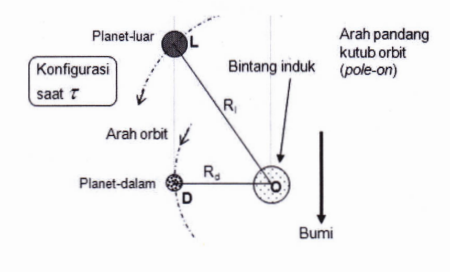
\includegraphics[width=0.6\textwidth]{no23.png}
\end{figure}
Bila rasio radius orbit planet dalam terhadap planet luar adalah 0,39685, hitunglah

\begin{enumerate}[(a)]
\item sudut fase dan fase planet luar dilihat dari planet dalam, dan sebaliknya,
\item busur sapuan planet dalam dan planet luar (segera setelah $\tau$) ketika okultasi yang sama (bukan pada kuadran lain) kembali terjadi.\\
\end{enumerate}


\textit{Jawaban: } 

\begin{figure}[ht!]
\centering
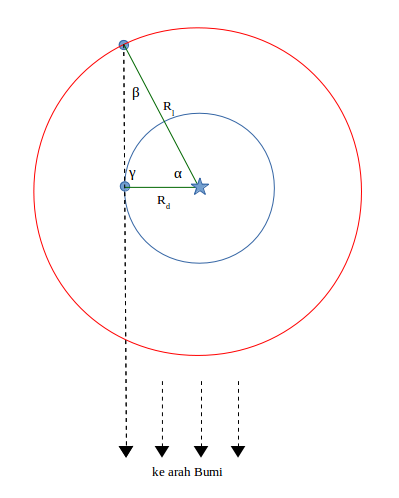
\includegraphics[width=0.4\textwidth]{23.png}
\end{figure}

Sudut $\alpha$ dapat dicari dengan,
\begin{eqnarray*}
\cos{\alpha} &=& \frac{R_{d}}{R_{l}}\\
\alpha &=& \arccos{0,39685}\\
\alpha &=& 66,61859612301\degree
\end{eqnarray*}

Karena $\gamma = 90\degree$, maka $\beta = 23,38140387699\degree$.

\begin{enumerate}[a)]
\item Berbeda dengan sudut elongasi yang terletak di pengamat, sudut fase ($\phi$) merupakan sudut yang terletak pada objek yang diamati. 

Fase ($q$) dapat dicari dari sudut fase ($\phi$) menggunakan persamaan,
$$q = \frac{1}{2} ( 1 + \cos{\phi})$$

\begin{itemize}
\item Menurut planet dalam, saat itu planet luar memiliki sudut elongasi $\beta = 23,38140387699\degree$ dan fase = 0,959. 

Planet luar terlihat ``hampir purnama'' menurut planet dalam.

\item Menurut planet luar, saat itu planet dalam memiliki sudut elongasi $\gamma = 90\degree$ dan fase = 0,5. 

Planet dalam terlihat ``setengah'' menurut planet luar; seperti Bulan terlihat saat quartir.
\end{itemize}

\item Dari hukum Kepler kita tahu bahwa perbandingan jarak rata-rata pangkat tiga dengan periode kuadrat selalu konstan untuk satu sistem; dalam hal ini kedua planet mengorbit bintang yang sama.
\begin{eqnarray*}
\frac{R_d^3}{T_d^2} &=& \frac{R_l^3}{T_l^2} = \text{konstan} \\
\left(\frac{T_d}{T_l}\right)^2 &=& \left(\frac{R_d}{R_l}\right)^3 \\
\frac{T_d}{T_l} &=& \left(\frac{R_d}{R_l}\right)^{3/2} \\
\frac{T_d}{T_l} &=& 0,24999975149 \simeq 0,25 = \frac{1}{4}
\end{eqnarray*}

Sepertinya pembuat soal sengaja membuat periode kedua planet merupakan kelipatan bilangan bulat. Artinya okultasi setelah $\tau$ akan terjadi lagi di kuadran yang sama `tepat' di titik yang sama pula, yaitu ketika planet luar sudah mengorbit tepat sekali, sedangkan planet dalam mengorbit tepat 4 kali. 
\begin{itemize}
\item Busur sapuan planet dalam $= 4 \times 360\degree = 1440\degree$
\item Busur sapuan planet luar $= 360\degree$
\end{itemize}


\end{enumerate}


\vspace{0.3cm}
\question Galaksi Bima Sakti memiliki tiga komponen populasi yaitu piringan, \textit{bulge}, dan halo. Diketahui massa total komponen piringan, $M_{\text{piringan}}= 6\times 10^{10} M_{\odot}$, dan luminositas totalnya, $L_{\text{piringan}}= 1,8\times 10^{10} L_{\odot}$. Hubungan antara luminositas dan massa untuk bintang deret utama mengikuti relasi:

$$\frac{L}{L_{\odot}} = \left( \frac{M}{M_{\odot}}\right)^\alpha$$

dengan nilai parameter $\alpha=4$. Hitunglah massa rata-rata bintang anggota populasi piringan di Bima Sakti.\\


\textit{Jawaban: } 

Hanya dengan data tersebut kita \textbf{tidak dapat} menentukan massa rata-rata bintang anggota populasi piringan Bima Sakti, bergantung pada fungsi distribusi massa bintangnya.
\begin{eqnarray*}
\sum_{i=1}^{N} {M_i} &=& 6\times 10^{10} = N \cdot \bar{M} \\
\sum_{i=1}^{N} {M_i^4} &=& 1,8\times 10^{10} \neq N \cdot \bar{M}^4
\end{eqnarray*}

Andaikan massa bintang semuanya sama, $M_i \equiv \bar{M}$, maka berlaku $\sum_{i=1}^{N} {M_i^4} = N \cdot \bar{M}^4$, sehingga
\begin{eqnarray*}
N \cdot \bar{M} &=& 6\times 10^{10}\\
N \cdot \bar{M}^4 &=& 1,8\times 10^{10}\\
\bar{M}^3 &=& 0,3\\
\bar{M} &=& 0,67 M_{\odot}  
\end{eqnarray*}


\vspace{0.3cm}
\question Kecepatan sudut rotasi diferensial Matahari dalam satuan derajat per hari dapat dinyatakan dengan rumus :

\begin{eqnarray*}
\centering
\Omega = 14,3 - 1,9 \sin^2 \phi - 2,5 \sin^4 \phi
\end{eqnarray*}

dengan $\phi$ adalah lintang heliografik. Dua kelompok bintik Matahari tersebut teramati berada bersamaan pada meridian tengah. Lintang heliografik kedua kelompok bintik Matahari masing-masing adalah $\phi_1=0\degree$ dan $\phi_2=+25\degree$. Keduanya bergerak sesuai dengan rumus kecepatan sudut di atas. Hitung berapa tahun lagikah kedua kelompok bintik Matahari tersebut bertemu kembali di meridian yang sama jika dilihat dari Bumi. Asumsikan gerak bintik Matahari tidak mengalami perubahan lintang heliografik.\\

\textit{Jawaban: } 

Dapat kita hitung kecepatan sudut masing-masing kelompok bintik Matahari:
$$\Omega_1 = 14,3 - 1,9 \sin^2{0} - 2,5 \sin^4{0} = 14,3 \qquad \text{derajat/hari}$$
dan
$$\Omega_2 = 14,3 - 1,9 \sin^2{25} - 2,5 \sin^4{25} = 13,514 \qquad \text{derajat/hari}$$

Untuk menentukan kapan mereka berada di meredian yang sama lagi, kita gunakan kecepatan sudut relatif antara keduanya,
\begin{eqnarray*}
\Omega_{rel} &=& \Omega_1 - \Omega_2\\
\frac{2 \pi}{T_{rel}} &=& \frac{2 \pi}{T_{1}} - \frac{2 \pi}{T_{2}} \qquad \text{rad/s} \quad \text{(sama seperti menentukan periode sinodis)}\\
\frac{360\degree}{T_{rel}} &=& 14,2 - 13,514 \qquad \text{derajat/hari}\\
T_{rel} &=& 458,093 \qquad \text{hari}\\
&=& 1,254 \qquad \text{tahun}
\end{eqnarray*}

Mereka akan bertemu lagi dibujur/meredian yang sama setiap 1,254 tahun. 

$^\ast$Apakah ketika itu terjadi, orang di Bumi dapat melihatnya? :)

$^\dagger$Ingat bahwa sebetulnya bintik Matahari bergerak perlahan ke arah ekuator dan lama-lama akan menghilang, digantikan bintik Matahari yang baru.


\end{questions}

%\centering{\--- SOAL SELESAI\---}


\vspace{5cm}
\begin{flushright}
Solusi ini dapat diperoleh di \url{http://ridlow.wordpress.com}
\end{flushright}
\end{document}
